\section{Chapter two}

  \vspace*{\fill}

  \begin{example}
    \centering
    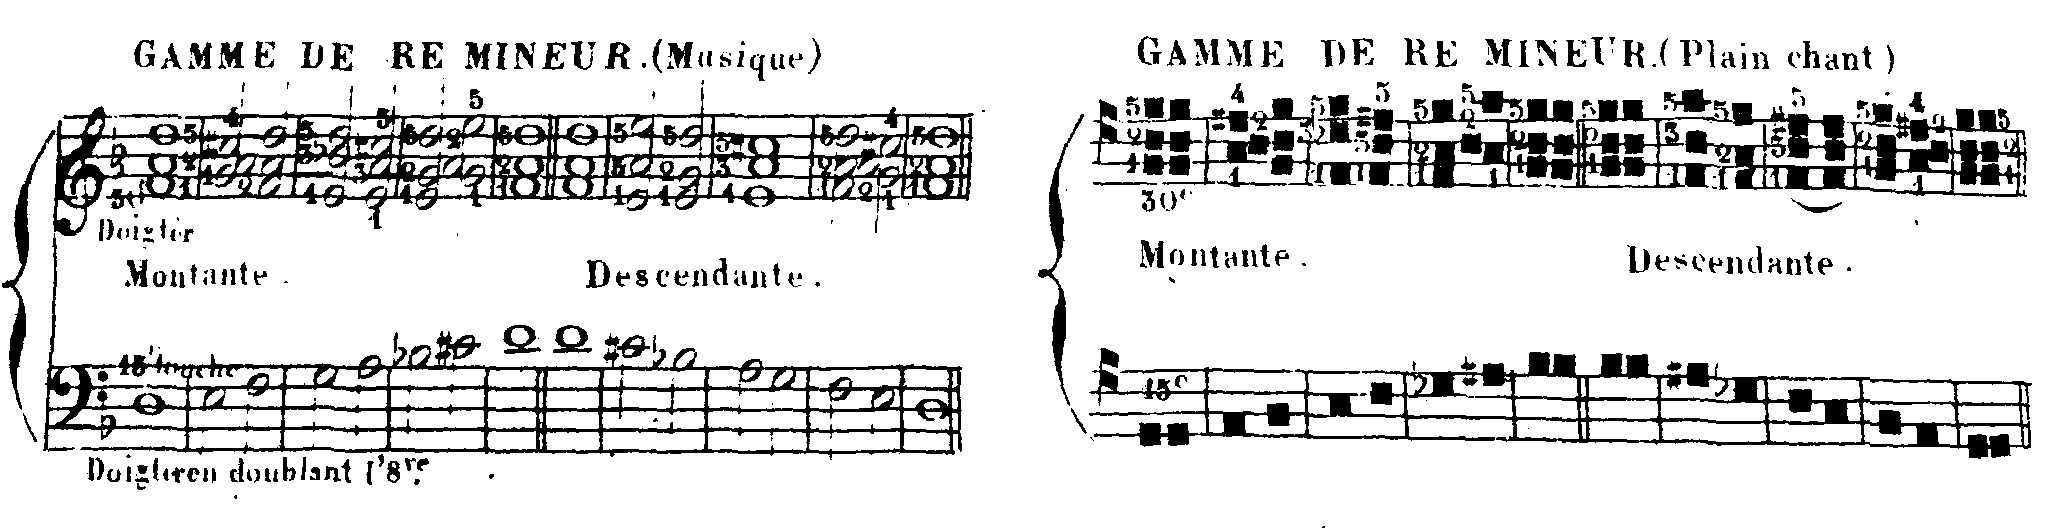
\includegraphics[width=\linewidth]{{c/2/ex/musiqueplainchant.jpg}}
    \caption{Bruneau, Duplicated music example, 1856}
    \label{mus:musiqueplainchant}
  \end{example}

  \vspace*{\fill}

  \begin{example}
    \centering
    \includely[nofragment,staffsize=16]{c/2/ex/danjouconservatoire}
    \caption{Danjou, `Choral' accompaniment, 1920s}
    \label{mus:danjou-conservatoire}
  \end{example}

  \vspace*{\fill}

  \clearpage

  \vspace*{\fill}

  \begin{example}
    \centering
    \includely[nofragment,staffsize=14]{c/2/ex/benoist/simplebass}\vspace{1cm}
    \includely[nofragment,staffsize=14]{c/2/ex/benoist/dissonancesbass}
    \caption{Benoist, Chant in bottom part, 1855}
    \label{mus:benoist-simple}
  \end{example}

    \vspace*{\fill}

  \begin{example}
    \centering
    \includely[nofragment,staffsize=14]{c/2/ex/benoist/simpletreble}\vspace{1cm}
    \includely[nofragment,staffsize=14]{c/2/ex/benoist/dissonancestreble}
    \caption{Benoist, chant in top, 1855}
    \label{mus:benoist-dissonances}
  \end{example}

  \vspace*{\fill}

  \clearpage

  \vspace*{\fill}

  \begin{example}
    \centering
    \includely[nofragment,staffsize=14]{c/2/ex/mine/fauxbourdon}
    \caption{Miné, `Faux Bourdon à la Pédale', 1845}
    \label{mus:mine-fauxbourdon}
  \end{example}

  \vspace*{\fill}

  \begin{example}
    \centering
    \includely[nofragment,staffsize=14]{c/2/ex/mine/laudasion}
    \caption{Miné, Accompaniment in filled notation, 1845}
    \label{mus:mine_lauda-sion}
  \end{example}

  \vspace*{\fill}

  \newpage

  \vspace*{\fill}

  \begin{example}
    \centering
    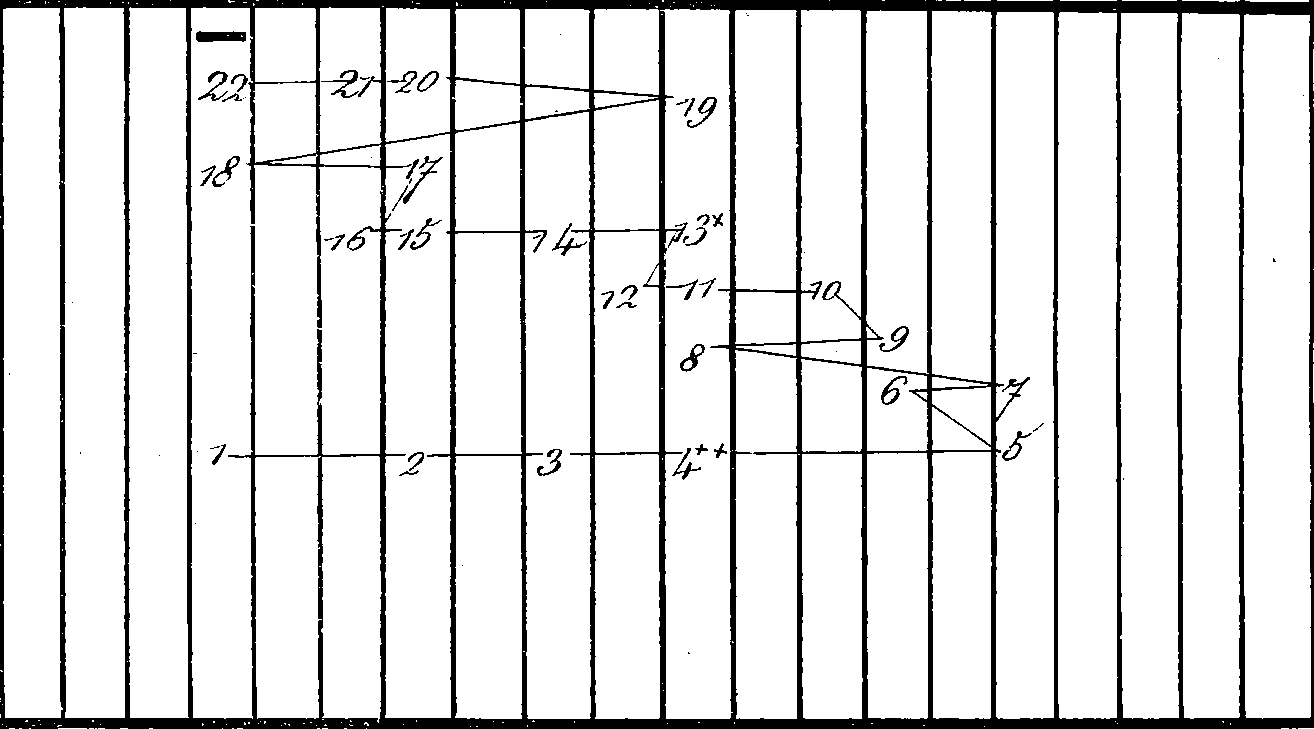
\includegraphics[width=.9\textwidth]{{c/2/ex/cabias.jpg}}
    \caption{`Orgue-Cabias' notation, 1834}
    \label{ex:cabias_notation}
  \end{example}

  \vspace*{\fill}

  \begin{example}
    \centering
    % \begin{lilypond}[staffsize=14]
    %   \new Staff \with {
    %       instrumentName="Christe"
    %     } {
    %     \relative c'  {
    %     \autoBeamOff
    %     \hide Staff.BarLine
    %     \hide Staff.TimeSignature
    %     a'8 a g a f g a d, c f g a g c b a gis a
    %     \undo \hide Staff.BarLine
    %     \bar "||"
    %   }
    % }
    % \end{lilypond}\\
    \begin{lilypond}[staffsize=16]
       \new Staff {
        \relative d {
        \clef tenor
        \autoBeamOff
        \hide Staff.BarLine
         \hide Staff.TimeSignature
        d8 f g a a a d c d a c b a gis a a g! f e f d a' f e d
        \undo \hide Staff.BarLine
        \bar "||"
        }
      }
    \end{lilypond}
    \caption{My transcription of \cref{ex:cabias_notation} (from \textit{Messe royale} by Dumont)}
    \label{ex:cabias_notation_transcription}
  \end{example}

  \vspace*{\fill}

\newpage

\vspace*{\fill}

\begin{example}
  \centering
  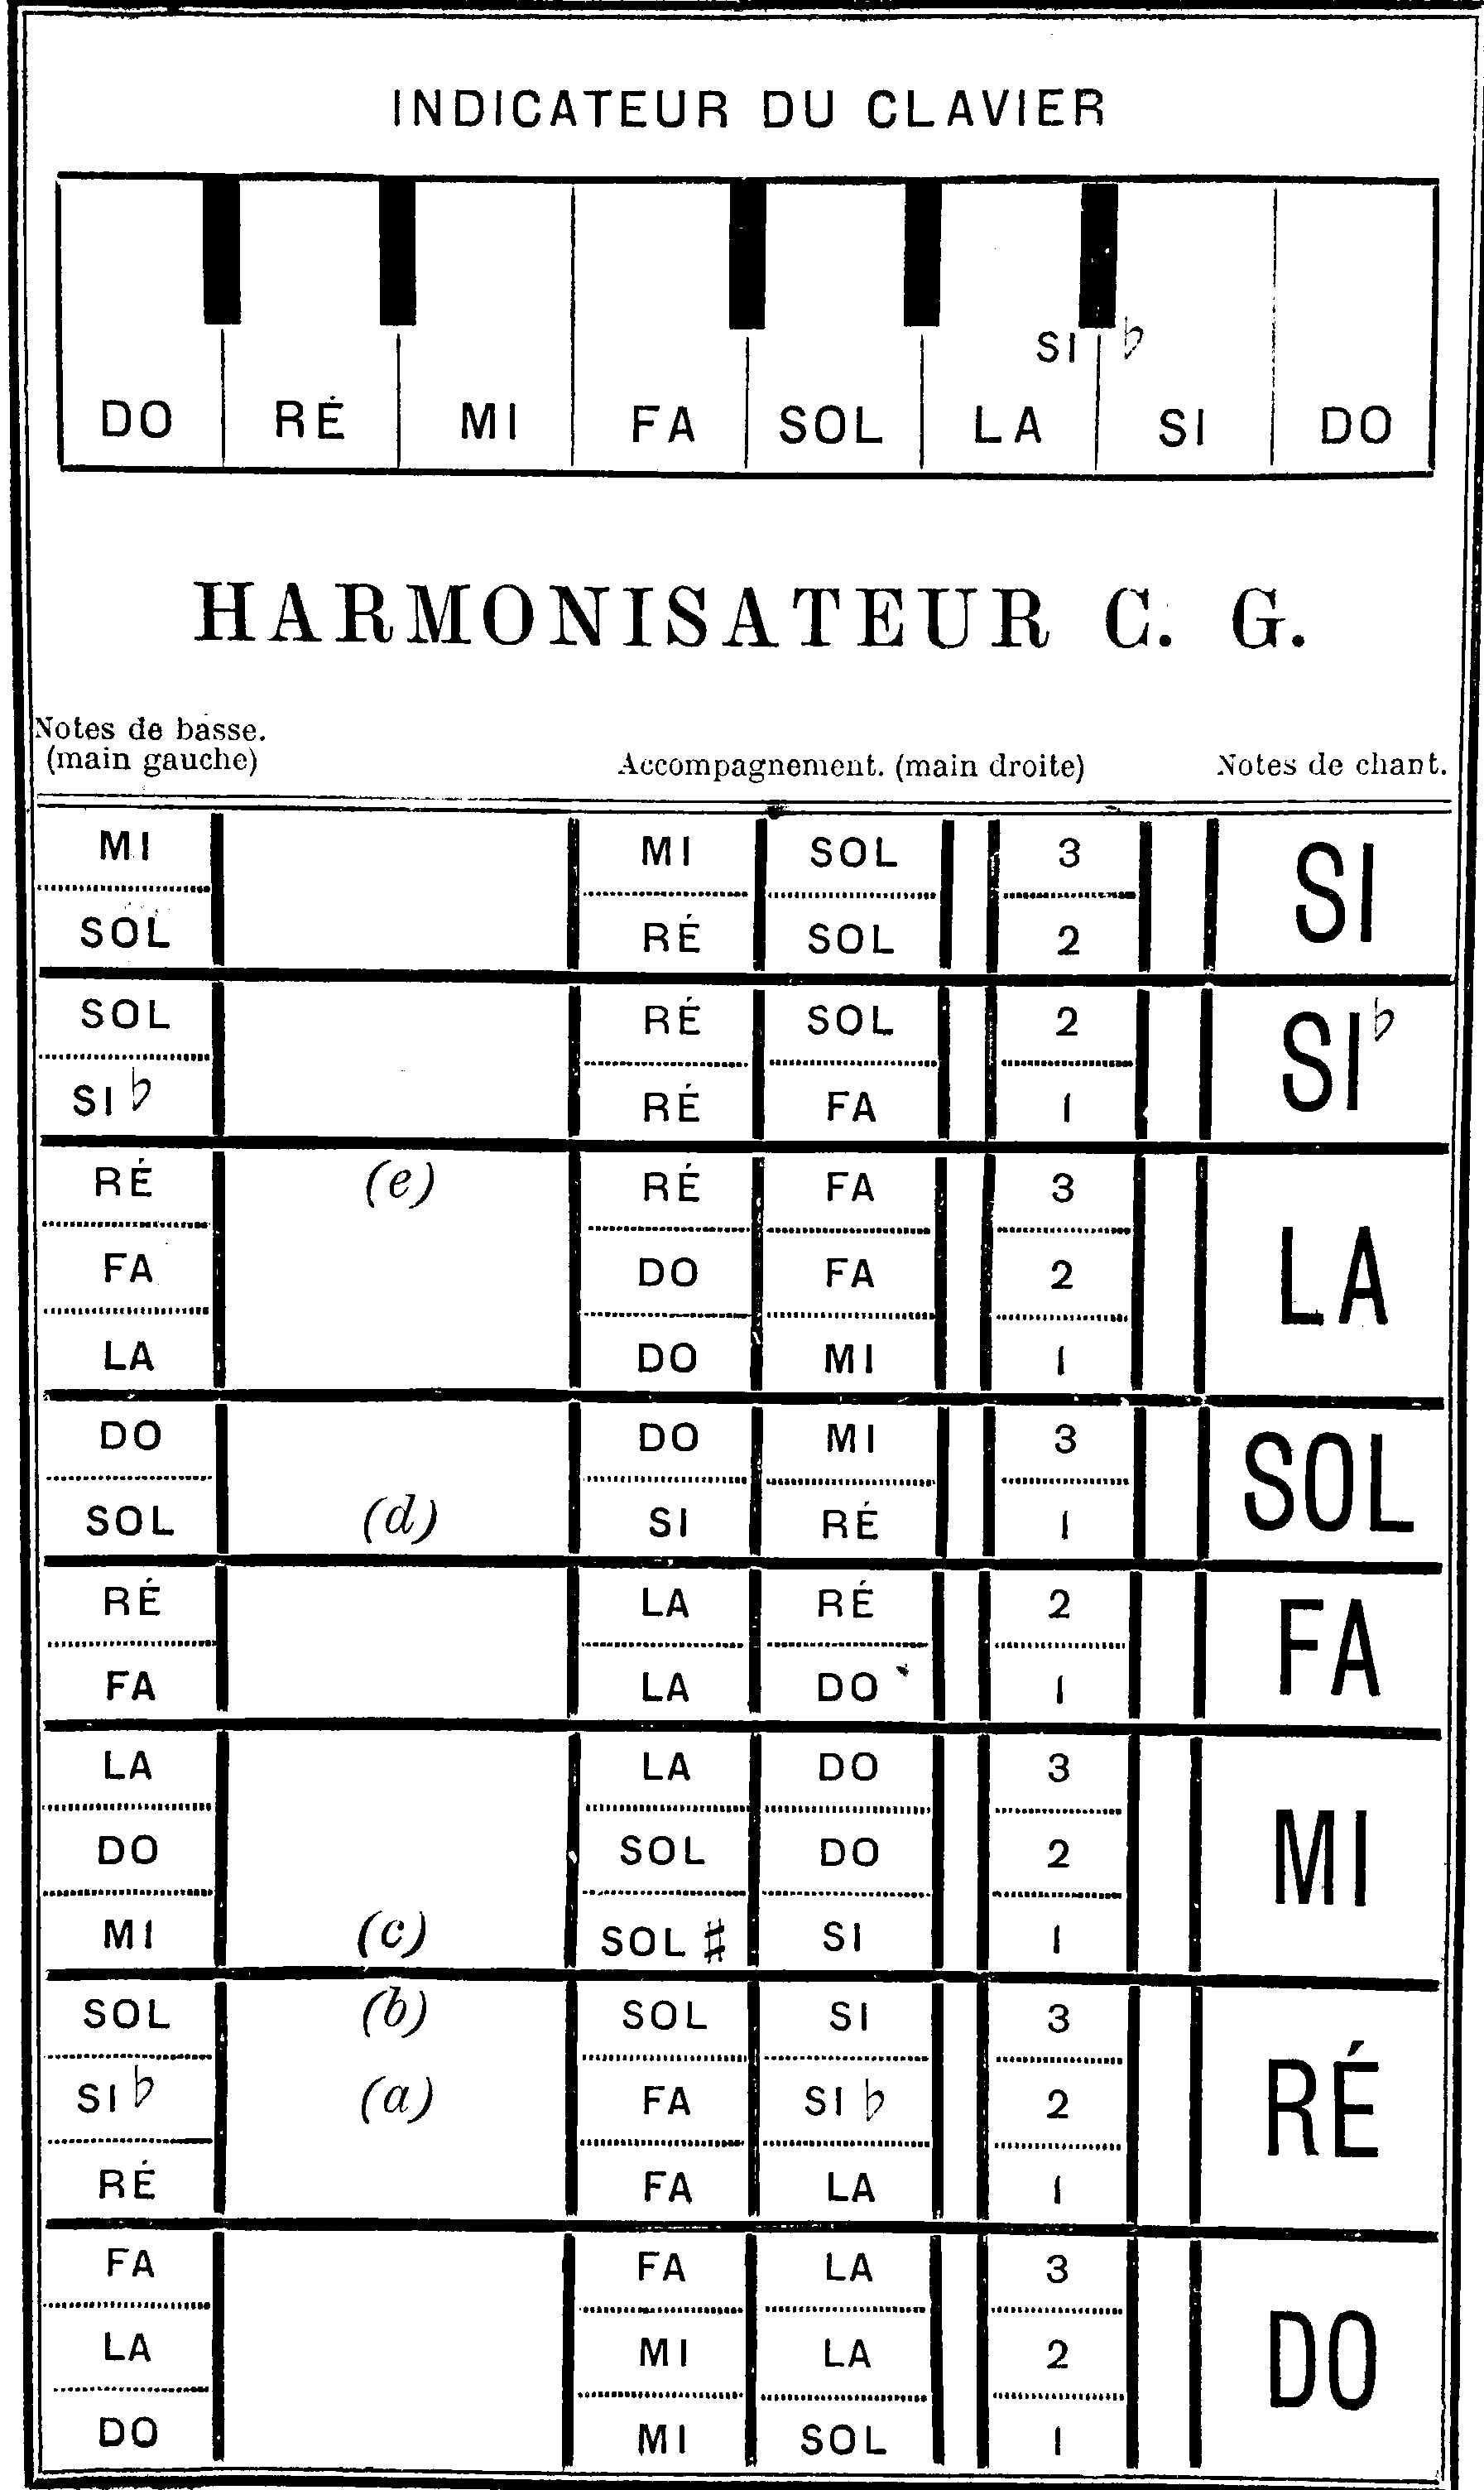
\includegraphics[width=.65\linewidth]{{c/2/ex/cg.jpg}}
  \caption{C.G., Table of chords, 1884}
  \label{fig:cg}
\end{example}

\vspace*{\fill}

\newpage

\vspace*{\fill}

\begin{example}
  \centering
  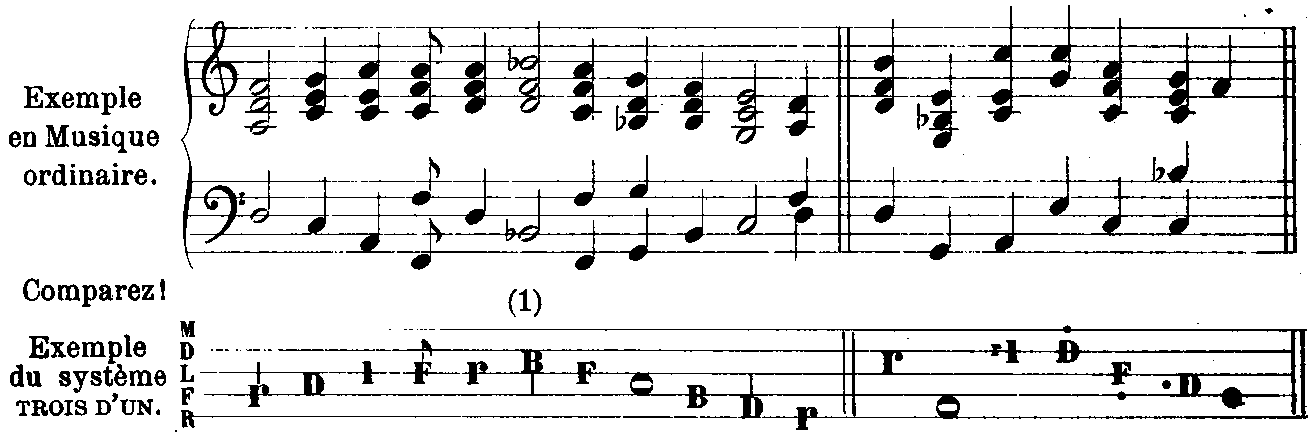
\includegraphics[width=\linewidth]{{c/2/ex/troisdun.png}}
  \caption{Dedun, The `three-in-one' system, 1889}
  \label{ex:dedun_troisdun}
\end{example}

\vspace*{\fill}

\newpage

\vspace*{\fill}

\begin{example}
  \centering
  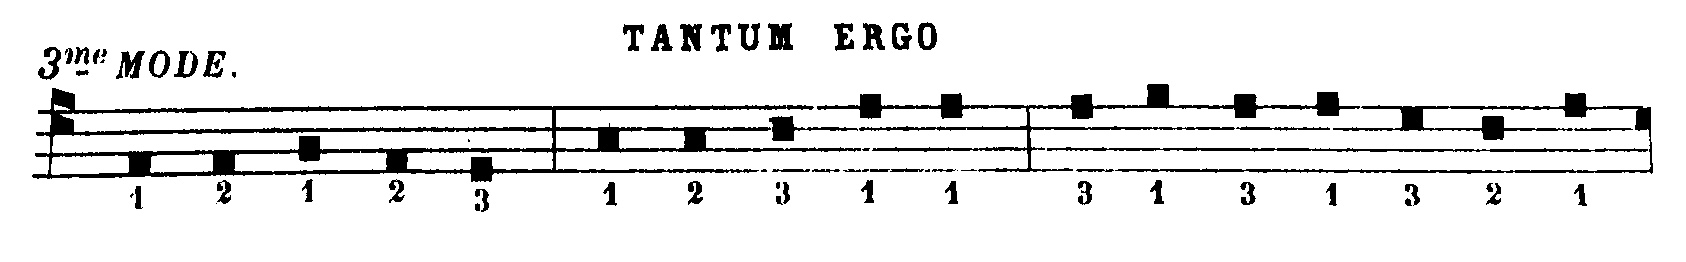
\includegraphics[width=\linewidth]{{c/2/ex/duvois_tantumergo.jpg}}
  \caption{Duvois, Numerical chords, 1844}
  \label{ex:duvois_tantumergo}
\end{example}

\vspace*{\fill}

\begin{example}
  \centering
  \includely[nofragment,staffsize=16]{c/2/ex/duvois/duvois}
  \caption{My realisation of \cref{ex:duvois_tantumergo}}
  \label{mus:duvois_realised}
\end{example}

\vspace*{\fill}

\newpage

\vspace*{\fill}

\begin{example}
  \centering
  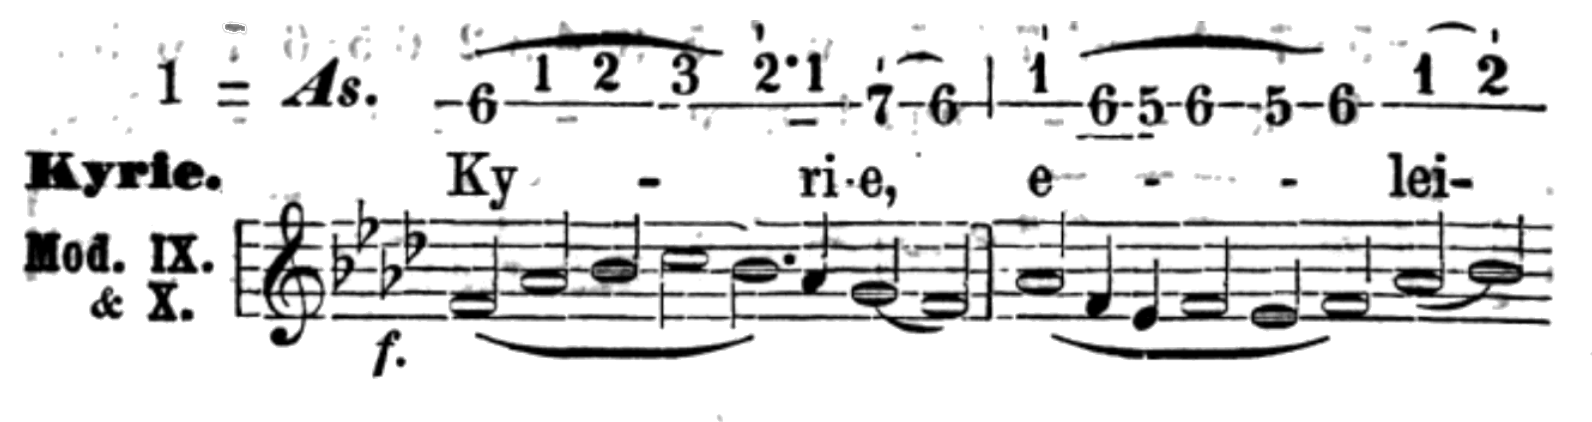
\includegraphics[width=\linewidth]{{c/2/ex/schneider_latinische_26.png}}
  \caption{Mayer, Numerical scale steps, 1867}
  \label{mus:mayer_numbers}
\end{example}

\vspace*{\fill}

\begin{example}
  \centering
  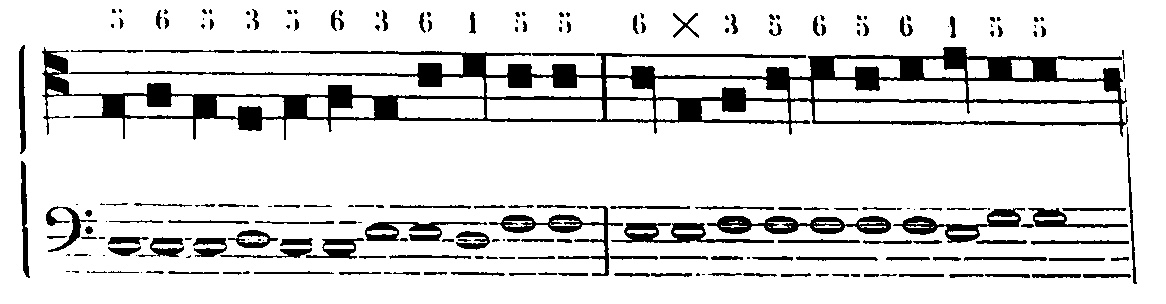
\includegraphics[width=\linewidth]{{c/2/ex/rousseau_figured.jpg}}
  \caption{Rousseau, Transcribed bass line from annotated `Veni creator', 1889}
  \label{ex:rousseau_figured}
\end{example}

\vspace*{\fill}

\newpage

\vspace*{\fill}

\begin{example}
  \centering
  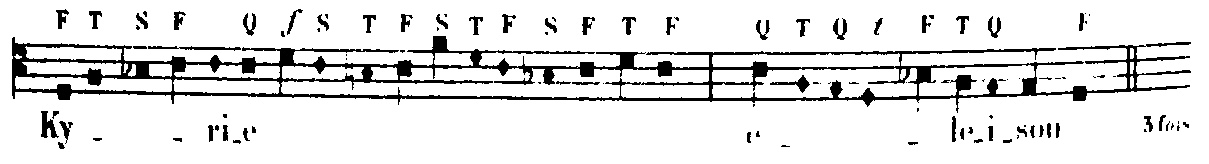
\includegraphics[width=\linewidth]{{c/2/ex/auzet.jpg}}
  \caption{Auzet, Annotated `Kyrie` from \emph{Missa de Angelis}, 1891}
  \label{ex:auzet_angelis}
\end{example}

\vspace*{\fill}

\begin{example}
  \centering
  \includely[nofragment,staffsize=16]{c/2/ex/auzet/auzet}
  \caption{My realisation of \cref{ex:auzet_angelis}}
  \label{mus:auzet_realised}
\end{example}

\vspace*{\fill}

\newpage

\vspace*{\fill}

\begin{example}
  \centering
  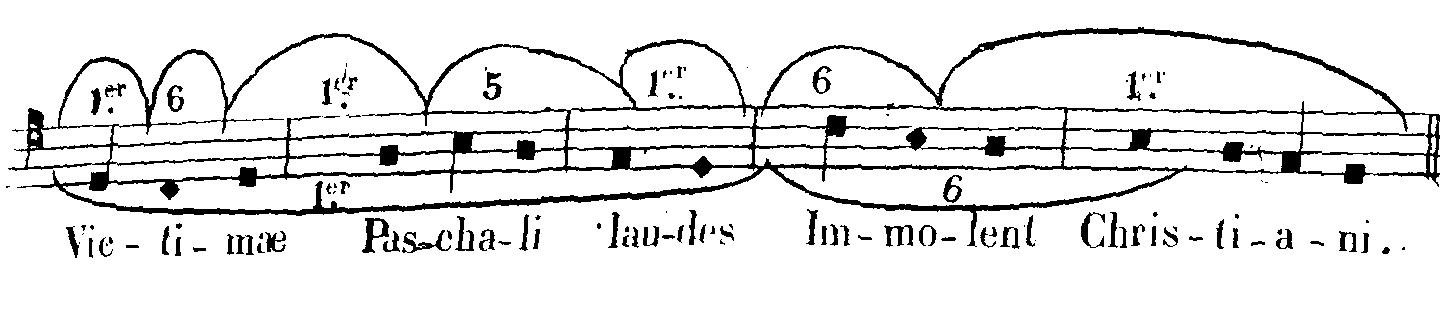
\includegraphics[width=.8\linewidth]{{c/2/ex/hanon_lines.jpg}}
  \caption{Hanon, Arcs display interpretation of melodic formul\ae{}, 1860}
  \label{ex:hanon_lines}
\end{example}

\vspace*{\fill}

\begin{example}
  \centering
  \includely[nofragment,staffsize=16]{c/2/ex/hanon/hanon}
  \caption{My realisation of \cref{ex:hanon_lines}}
  \label{mus:hanon_realised}
\end{example}

\vspace*{\fill}

\begin{landscape}

  \vspace*{\fill}

  \begin{example}
    \centering
    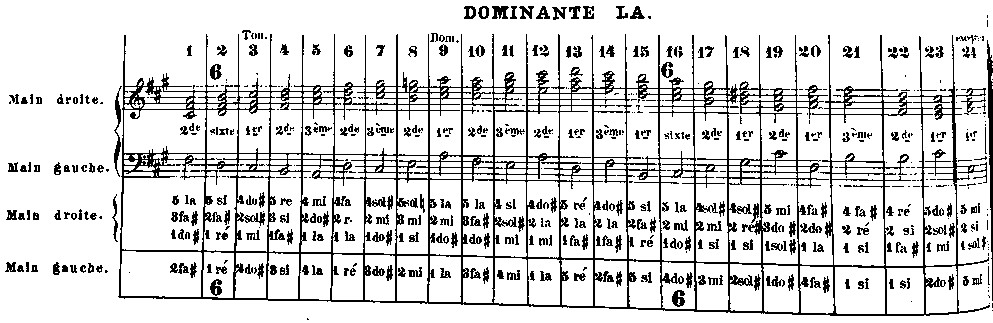
\includegraphics[width=.7\linewidth]{{c/2/ex/allard_table.jpg}}
    \caption{Allard, Set of chords for the third mode, 1880}
    \label{ex:allard_table}
  \end{example}

  \vspace*{\fill}

  \begin{example}
    \centering
    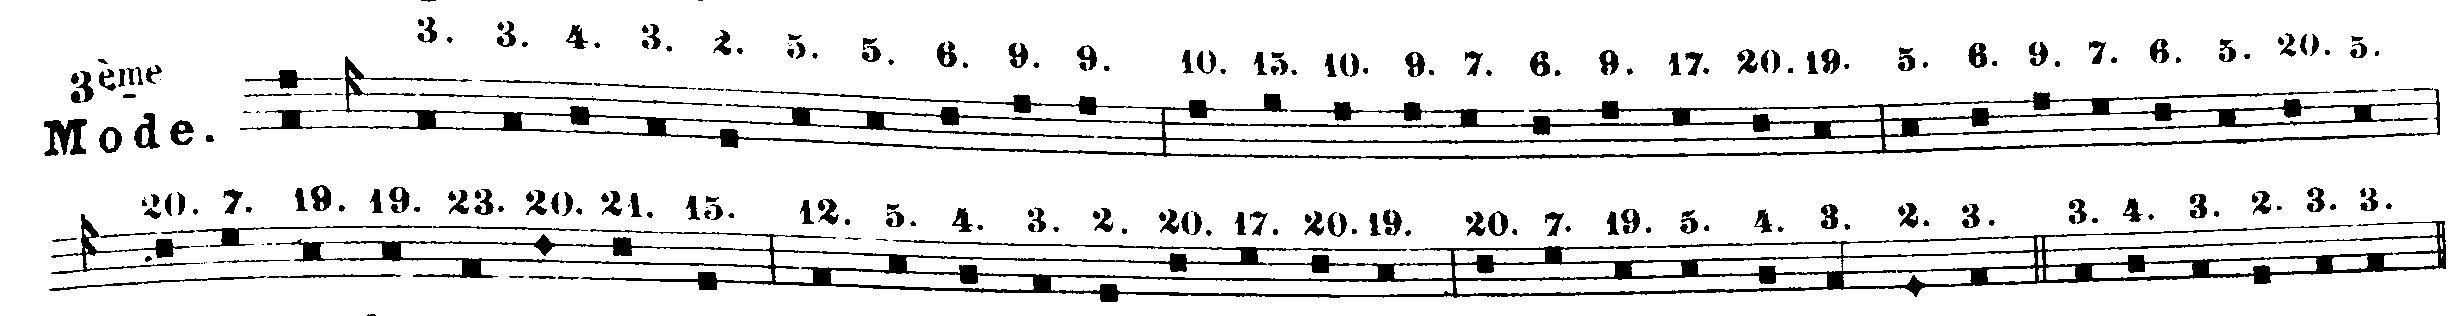
\includegraphics[width=.7\linewidth]{{c/2/ex/allard_pangelingua.jpg}}
    \caption{Allard, Numerals indicate chords in \cref{ex:allard_table}, 1880}
    \label{ex:allard_pangelingua}
  \end{example}


  \vspace*{\fill}

\end{landscape}

\vspace*{\fill}

\begin{example}
  \centering
  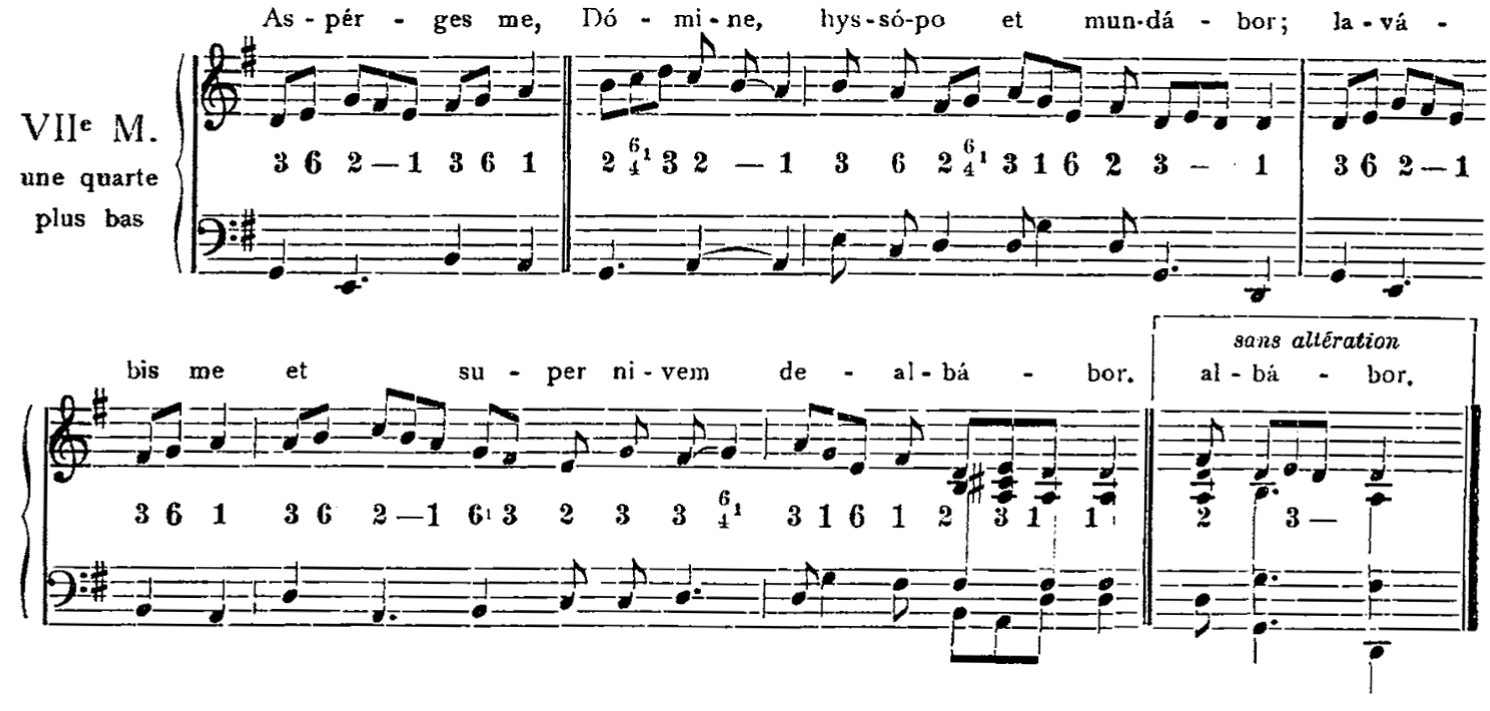
\includegraphics[width=\linewidth]{{c/2/ex/brune_asperges.jpg}}
  \caption{Brune, Annotations transcribed, 1903}
  \label{ex:brune_figured}
\end{example}

\vspace*{\fill}

\begin{example}
  \centering
  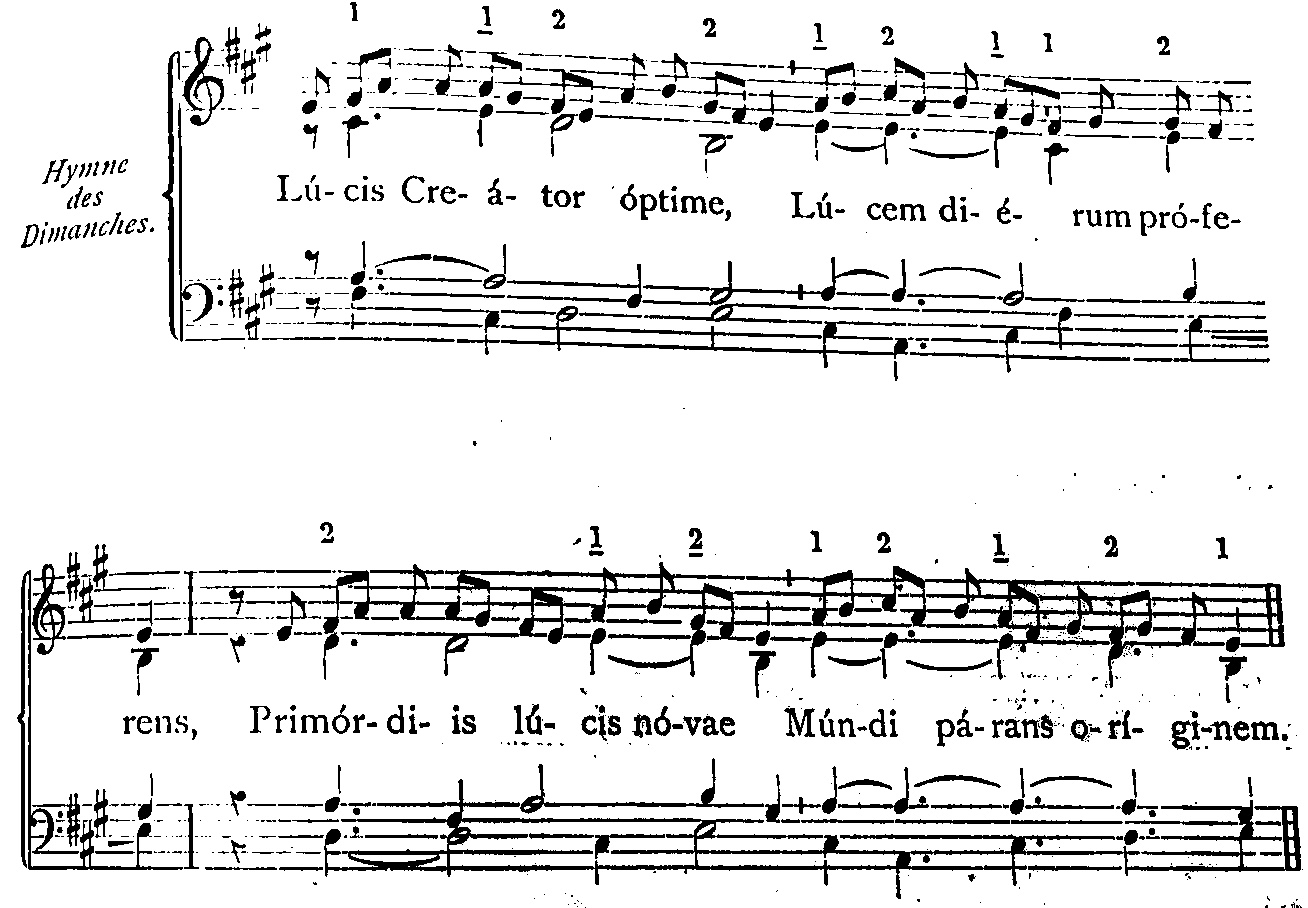
\includegraphics[width=.8\linewidth]{{c/2/ex/aumonbiret_figured.jpg}}
  \caption{Aumon and Biret, Annotations transcribed, 1926}
  \label{ex:aumonbiret_figured}
\end{example}

\vspace*{\fill}

\newpage

\vspace*{\fill}

\begin{example}
  \centering
  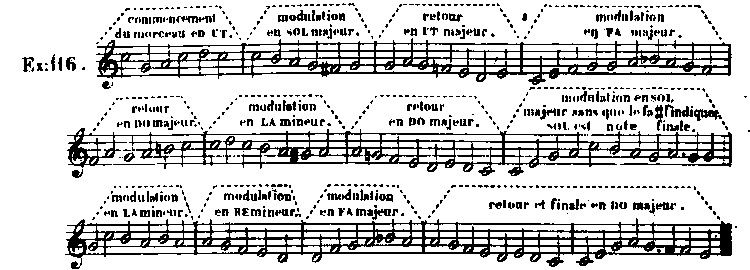
\includegraphics[width=\linewidth]{{c/2/ex/battmann_34.jpg}}
  \caption{Battmann, Modulation towards phrase-end, 1855}
  \label{mus:battmann_34}
\end{example}

\vspace*{\fill}

\begin{example}
  \centering
  \includegraphics[width=.8\linewidth]{c/3/ex/gevaert_notation.png}
  \caption{Gevaert, Stretched breve and sharped cadence, 1856}
  \label{mus:gevaert_notation}
\end{example}

\vspace*{\fill}

\newpage

\vspace*{\fill}

\begin{example}
  \centering
  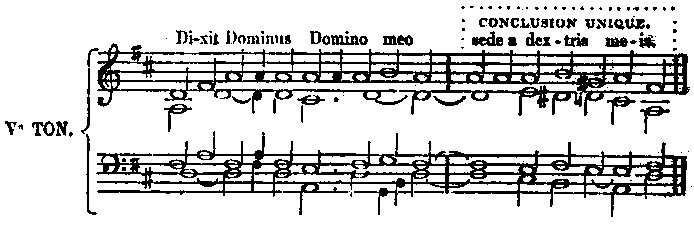
\includegraphics[width=\linewidth]{{c/2/ex/janssen_tone5.jpg}}
  \caption{Janssen, Fifth psalm tone, 1845}
  \label{mus:janssen_tone5}
\end{example}

\vspace*{\fill}

\begin{landscape}

  \vspace*{\fill}

  \begin{example}
    \centering
    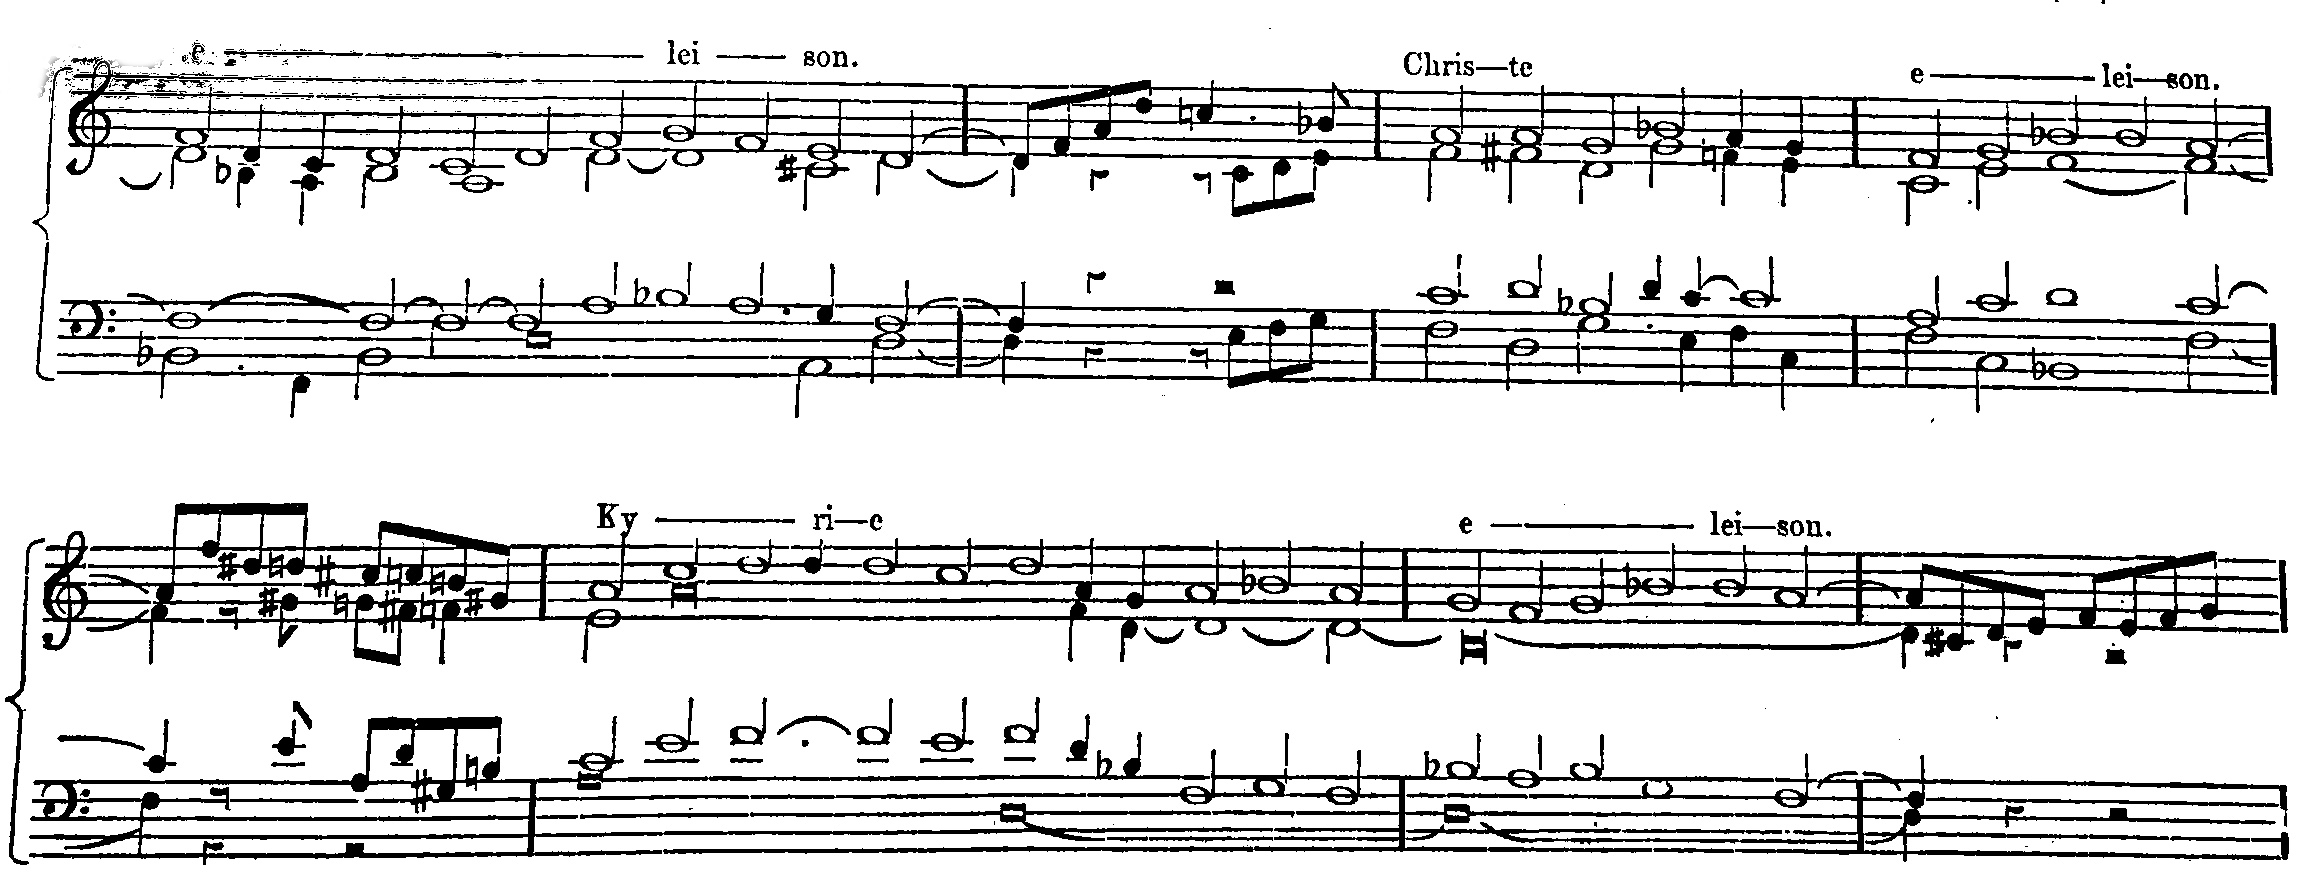
\includegraphics[width=.7\linewidth]{c/2/ex/duval_madness.jpg}
    \caption{Duval, Rinck-inspired interlude, 1845}
    \label{mus:duval_madness}
  \end{example}

  \vspace*{\fill}

\end{landscape}

\vspace*{\fill}

\begin{example}
  \centering
  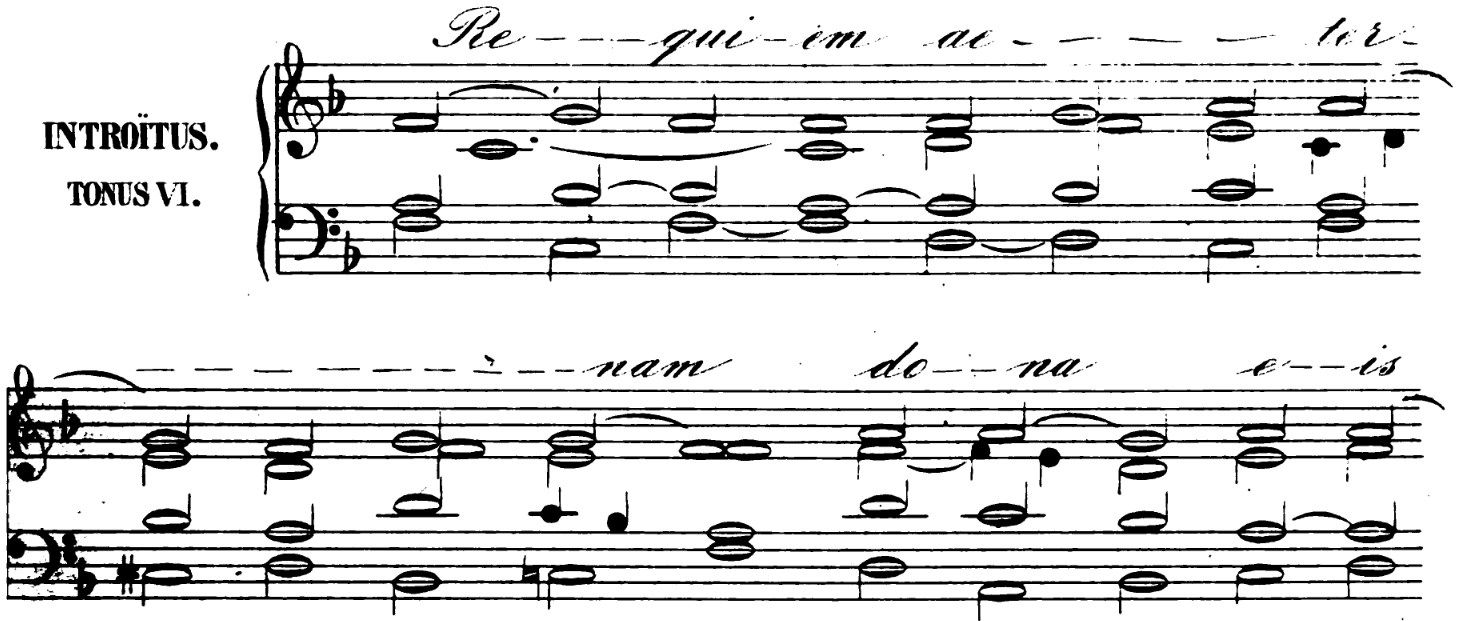
\includegraphics[width=\linewidth]{{c/1/ex/hageman_requiem_65.png}}
  \caption{Hageman, Chromatic harmony in Janssen's style, 1859}
  \label{mus:hageman_requiem}
\end{example}

\vspace*{\fill}

\newpage

\vspace*{\fill}

\begin{example}
  \centering
  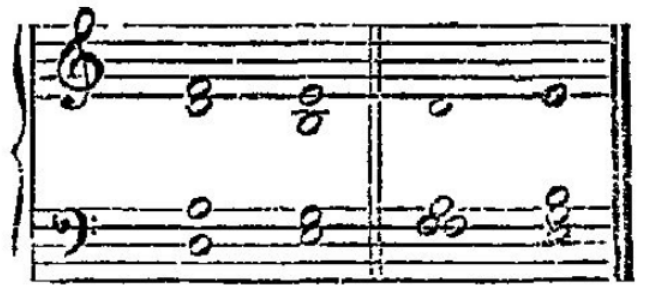
\includegraphics[width=.4\linewidth]{{c/2/ex/niedermeyer_deuterus_natural.png}}
  \caption{Niedermeyer, Diatonic deuterus cadence, 1859}
  \label{mus:niedermeyer_deuterus_natural}
\end{example}

\vspace*{\fill}

\begin{example}
  \centering
  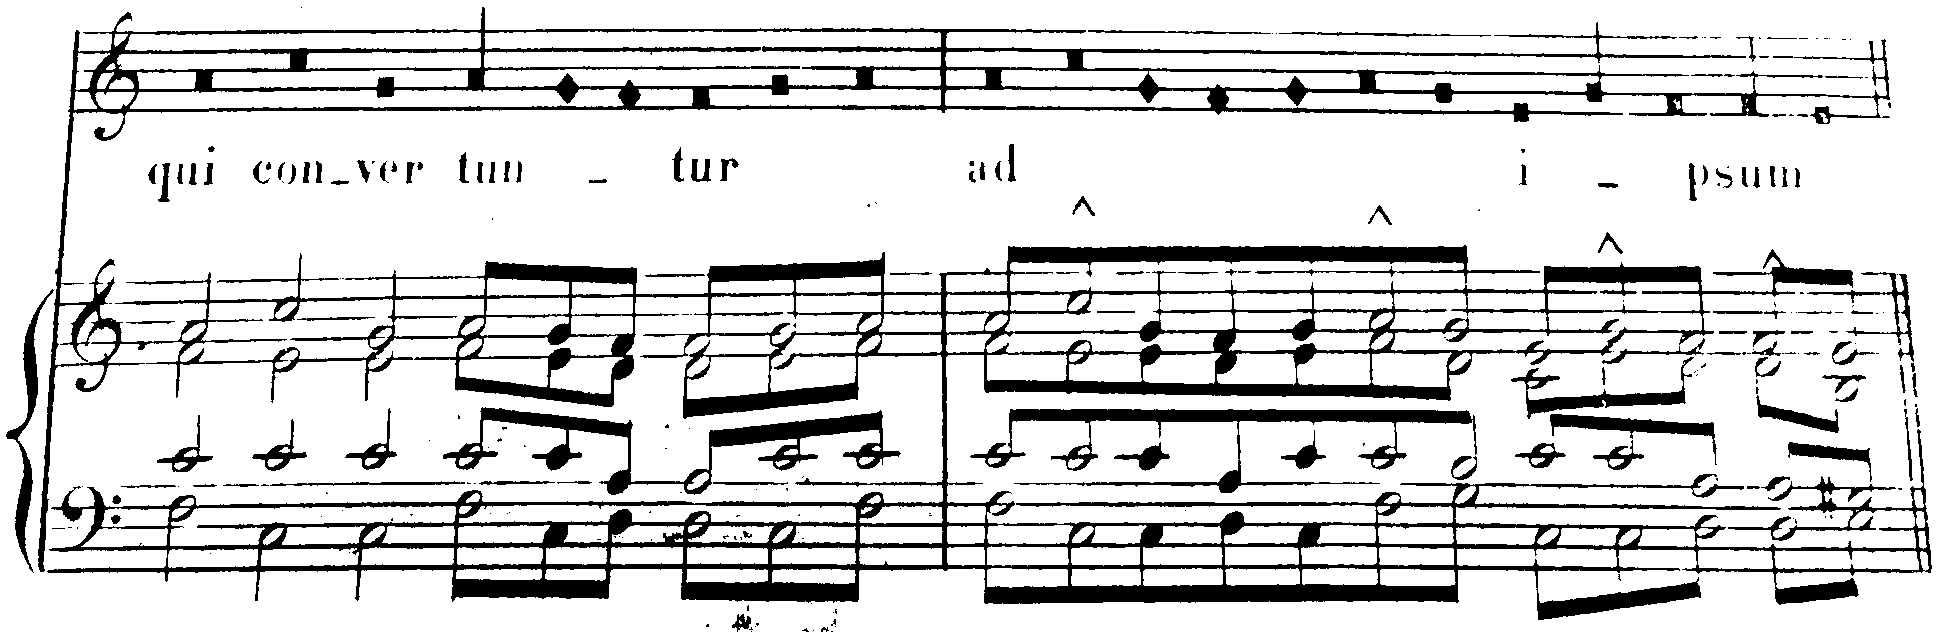
\includegraphics[width=\linewidth]{{c/2/ex/schmitt_deuterus.jpg}}
  \caption{Schmitt, Sharped deuterus cadence, 1864}
  \label{mus:schmitt_deuterus}
\end{example}

\vspace*{\fill}

\begin{landscape}

\vspace*{\fill}

\begin{example}
  \centering
  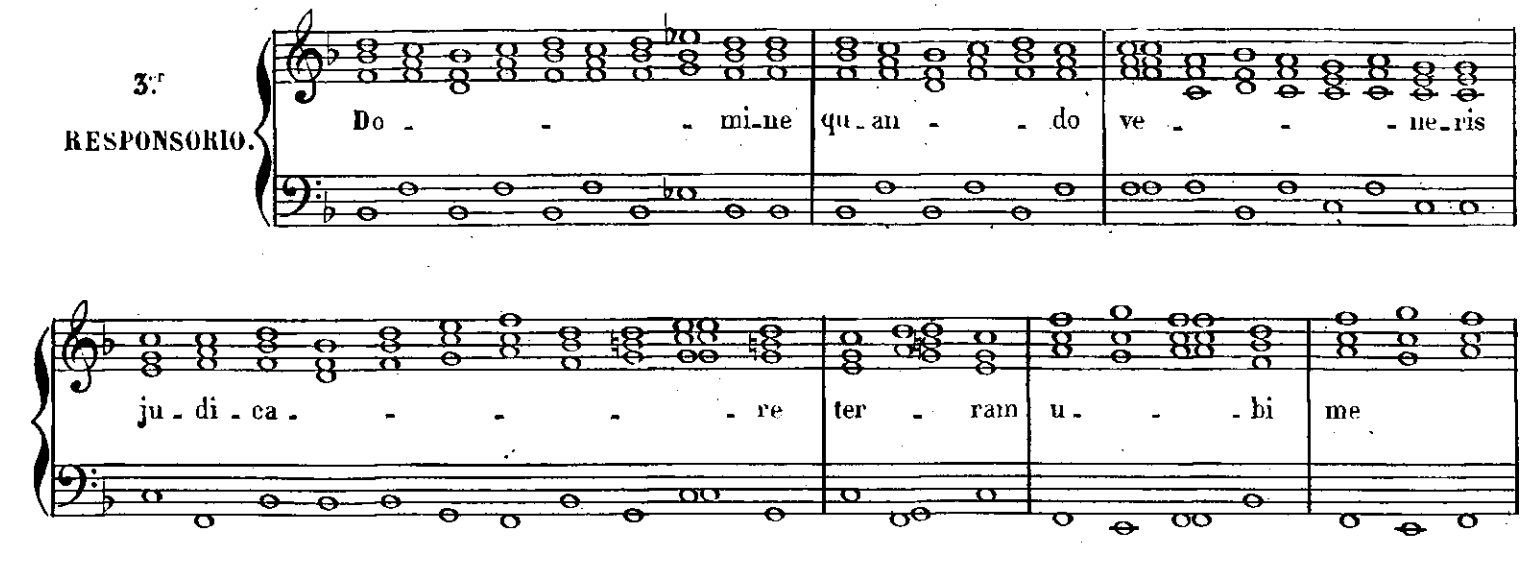
\includegraphics[width=.8\linewidth]{{c/2/ex/ovejero.png}}
  \caption{Ovejero, Chordal style, 1876}
  \label{mus:ovejero}
\end{example}

\vspace*{\fill}

\end{landscape}

\vspace*{\fill}

\begin{example}
  \centering
  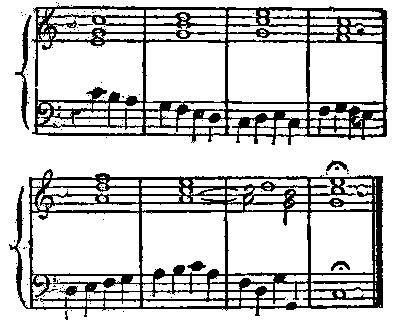
\includegraphics[width=.45\linewidth]{{c/2/ex/boulanger_lent.jpg}}
  \caption{Boulanger, Example of \textit{Lent} accompaniment, 1860}
  \label{mus:boulanger_lent}
\end{example}

\vspace*{\fill}

\begin{example}
  \centering
  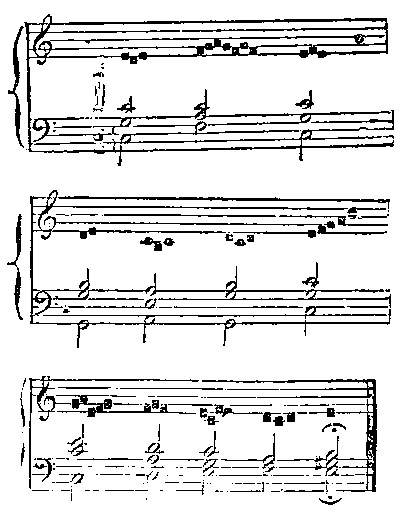
\includegraphics[width=.45\linewidth]{{c/2/ex/nisard_vif.jpg}}
  \caption{Nisard, Example of \textit{Vif} accompaniment, 1860}
  \label{mus:nisard_vif}
\end{example}

\vspace*{\fill}

\newpage

\vspace*{\fill}

\begin{example}
  \centering
  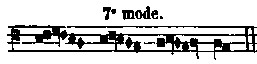
\includegraphics[width=.4\linewidth]{{c/2/ex/nisard_chant.jpg}}
  \caption{Chant example provided by Nisard, 1860}
  \label{mus:nisard_chant}
\end{example}

\vspace*{\fill}

\begin{example}
  \centering
  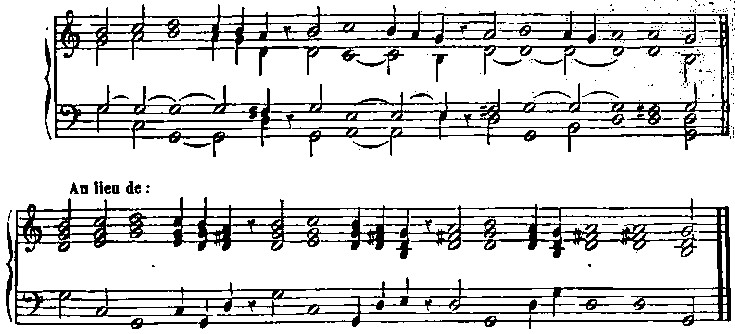
\includegraphics[width=.8\linewidth]{{c/2/ex/nisard_counterpoint.jpg}}
  \caption{Nisard, \cref{mus:nisard_chant} in sustained and chordal styles, 1860}
  \label{mus:nisard_counterpoint}
\end{example}

\vspace*{\fill}

\begin{landscape}

  \vspace*{\fill}

  \begin{example}
    \centering
    \includegraphics[width=.65\linewidth]{{c/2/ex/populus_congress.png}}
    \caption{Populus, Example from the Paris congress, 1860}
    \label{mus:populus_congress}
  \end{example}

  \vspace*{\fill}

\end{landscape}

\vspace*{\fill}

\begin{example}
  \centering
  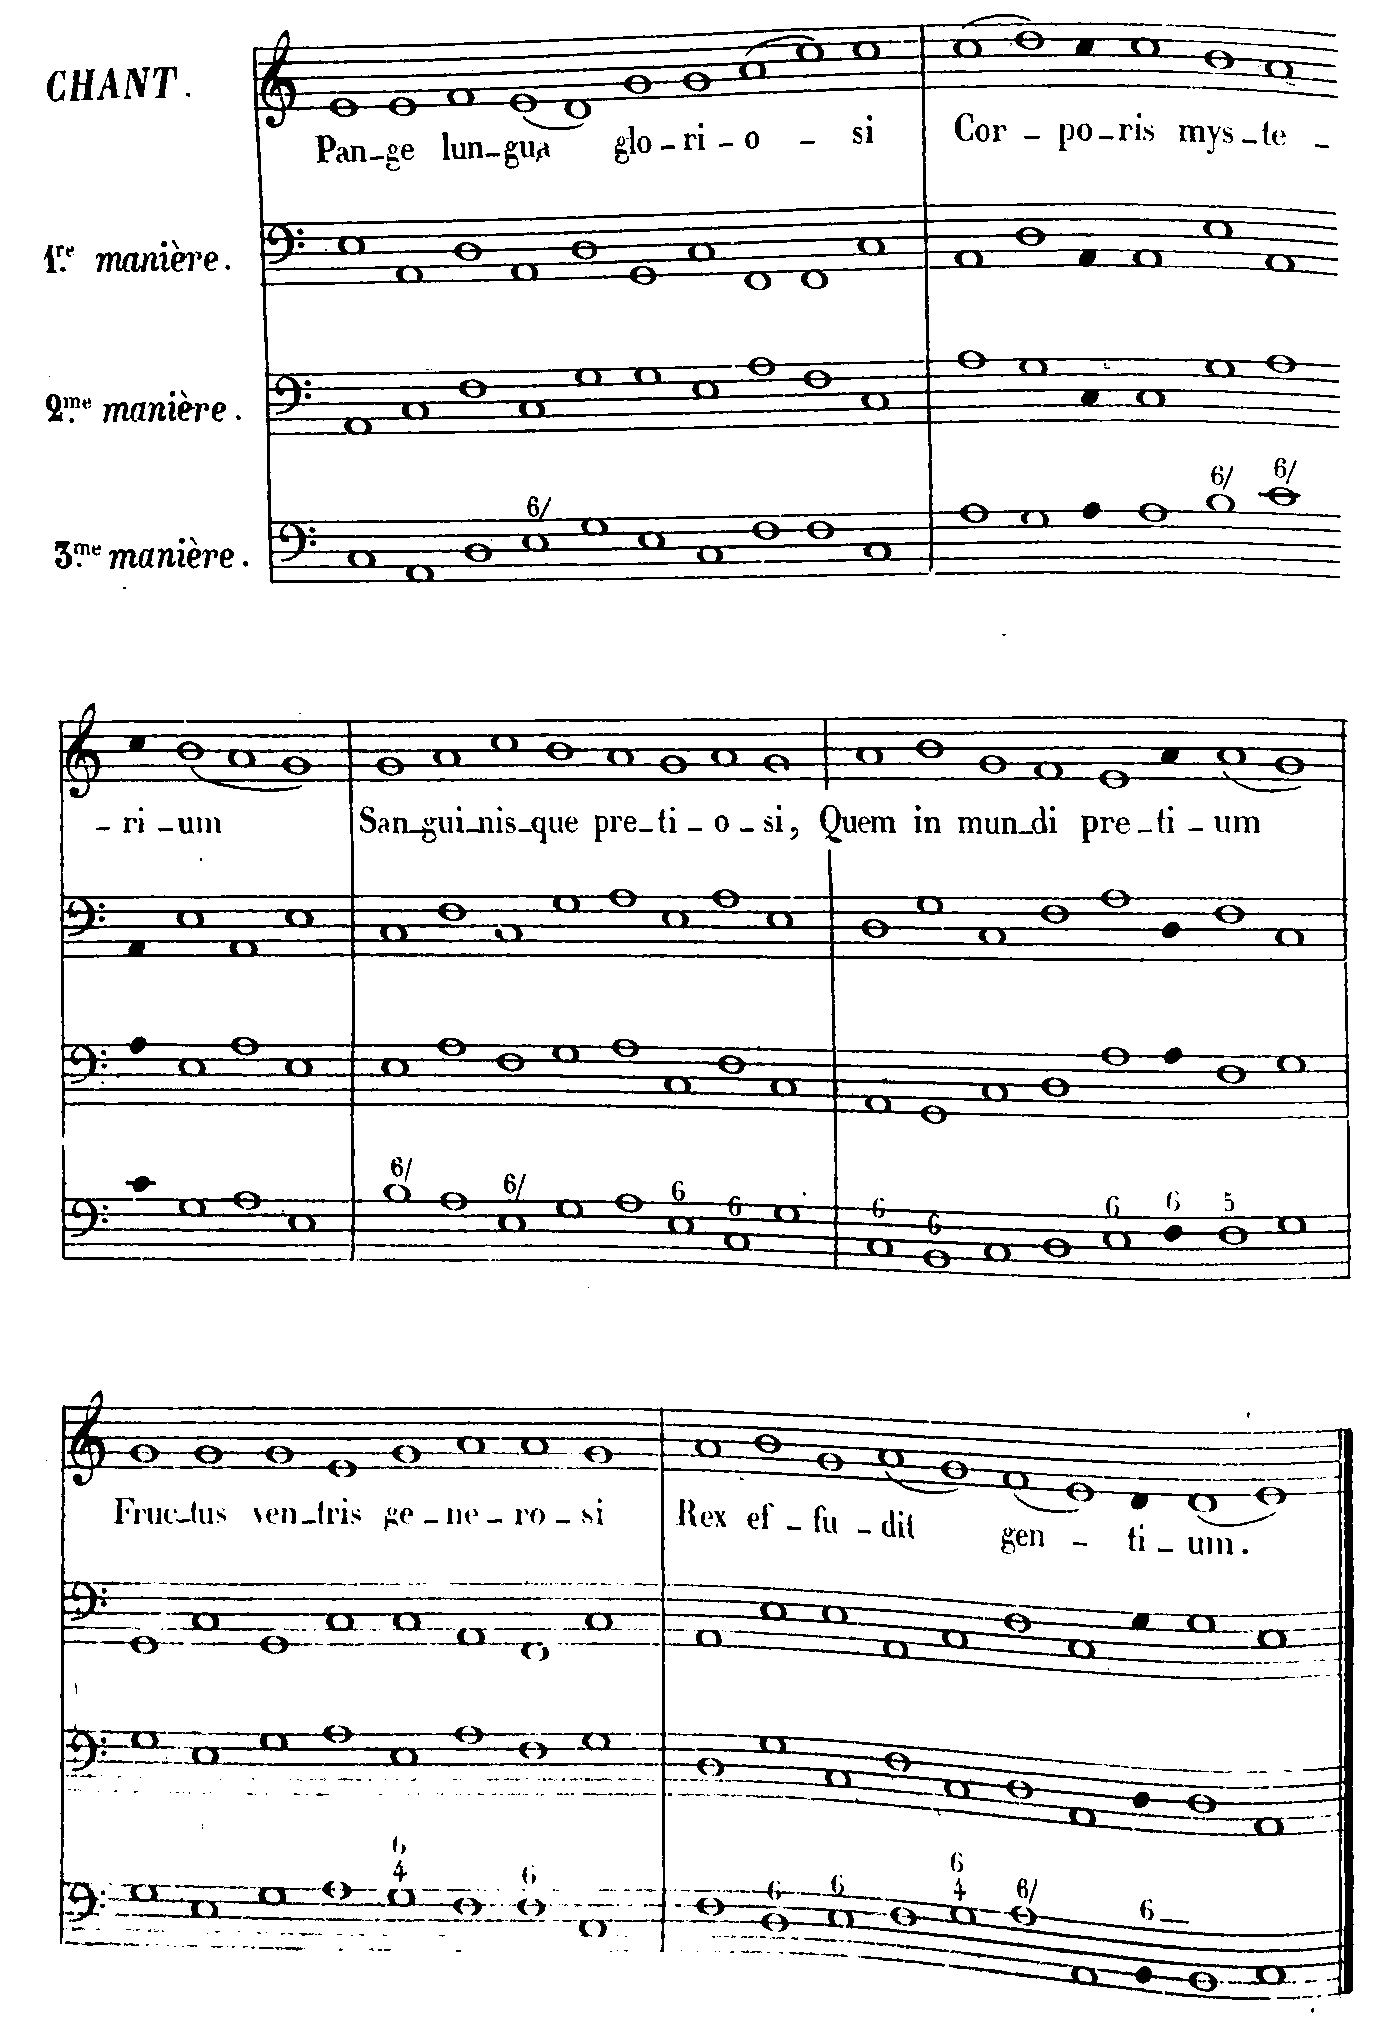
\includegraphics[width=.75\linewidth]{{c/2/ex/populus_three_bass.jpg}}
  \caption{Populus, Comparative bass lines, 1863}
  \label{mus:populus_three_bass}
\end{example}

\vspace*{\fill}

\newpage
